\chapter{Кий – спутник Геракла}

Самое время снова колебать основы.

Вспомним начало этой книги, там где про варягов. Откуда родом Рюрик?

\begin{quotation}
иже начася от Рюрика, его же выше рекохом, иже прииде из Варяг в Великий Нов Град со двомя братома своима и с роды своими, иже бе; от племени Прусова, по его же имени Пруская земля именуется; Прус же брат бысть единоначальствующаго на земли Римскаго Кесара Августа.
\end{quotation}

И ранее я рассуждал о том, что народ Прусов жил на юге Балтийского моря, а на то есть основания, по разным источникам. 

Теперь про Кия вспомним несторовы слова:

\begin{quotation}
Аще бо был перевозник Кый, то не бы ходил к Царюграду; но сий Кий княжаше в роду своем; и приходившю ему к царю не свемы, но токмо о сем вемы, якоже сказають, яко велику честь приял есть от царя, которого не вем и при котором приходи цари. [далее о хождении Кия возле Дуная]
\end{quotation}

Что же Нестор? Он не знает, при каком царе, но Кий, княжащий в своем роде, ходил в Царьград, Константинополь, и был принят с почестями.

Ниже я приведу выдержку из «Географии»\cite{strabon01} Страбона, книги 12, главы 4:

\begin{quotation}
1. Бифиния граничит с востока Пафлагонцами, Мариандинами и частью Епиктетов, с севера Понтским морем от устьев Сангария до входа при Византии и Халкеодне, с запада Пропонтидою, и наконец с юга Мисией и так называемой приобретенной Фригией, которая называется также Геллеспонтской Фригией.

2. Здесь при входе в Понт лежал Халкедон, колония Мегарцев, деревня Хризополь и храм Халкедоний. В окрестностях города не высоко над морем имеется источник Азарития, в которм водятся небольшие крокодилы. Далее следует морской берег Халкедонцев, так называемый залив Астакен, составляющий часть Пропонтиды; в нем построена Никомедея, названная так по имени бифинского царя, основавшего этот город.

Многие лица названы были таким же именем, благодаря  славе первого, подобно тому, как и Птолемеи. В том же заливе был и город Астак, колония Магарцев, Афинян и позже Дойдался; от этого города и залив получил свое название. Он был срыт по распоряжению Лизимаха, а жителей его перевел в Никомедею основатель последней.

3. С заливом Астакеном соединяется другой залив, лежащий далее к востоку; в нем есть Прусия, называвшаяся в древности Кием. Кий разрушен Филиппом, сыном Деметрия и отцом Персея. Он подарил место Прусии\footnote{Prusias, Προυσίας}, сыну Зелы, который вместе с этим городом разрушил соседнюю Мирлею, лежавшую недалеко и от Прусы. Восстановивши оба города из развалин, Прусия назвал один из них, Кий, по своему имени Прусиадою, а другой Мирлею, по имени жены Апамеею. 

Это тот самый Прусия, который принял Аннибала, бежавшего туда после поражения Антиоха, и который по договору отделил Фригию при Геллеспонте Атталикам; в древности она называлась Малой Фригией, а те назвали ее Приобретенной. Над Прусиадою возвышается гора, которую называют Арганфонием. 

Жители повествуют, что Гила\footnote{Он же Иолай, любовник Геракла.}, один из спутников Геракла, плывший вместе с ним на корабле Арго, вышел здесь на берег к источнику и был похищен нимфами, а Кий будто бы, также спутник Геракла и также плывший с ним из Колхиды, остался здесь и основал город, названный его именем. 

И теперь еще у Прусиев совершается празднество и блуждание по горам, причем устраиваются процессии и вызывается Гила, и как будто для отыскания его выходят из леса. Так как Прусиеи держали себя по отношению к Римлянам дружелюбно, то они сохранили свою свободу; напротив Анамеи (Апамеи?) приняли римских колонистов. Пруса лежит у Мисийского Олимпа; это – город с хорошим управлением, пограничным с Фригийцами и Милийцами, колония Прусии, воевавшего с Крезом.
\end{quotation}

Вот это да! Оказывается, Кий – а я не сомневаюсь, что это наш родной, летописный князь Кий – участвовал вместе с Гераклом в походе аргонавтов, и основал город в Малой Азии, город Кий (Kίος Kios), который потом был переименован в Прусу – ныне это известный турецкий город Бурса\footnote{Ученые, впрочем, отождествляют с городом Кием развалины в 30 километрах от Бурсы. Не так далеко от Бурсы еще и турецкий город Ялова, вполне славянское название, дескать, «еловый», или деревня «еловая». В окрестностях там растут хвойные деревья.}. Не так уж далеко от Троады. А что напротив Бурсы, 60 километров на север по Мраморному морю? А Константинополь. 

Ну так и наш Нестор пишет, что ходил Кий в Константинополь, только не вем при каком царе. Но ходил. Именно оттуда наверное и к Дунаю пошел – что гораздо ближе, нежели от города Киева по Днепру да через море двигаться.

И как страна, где город Кий, он же Пруса или Бурса находится, называлась в давние времена? Фригия, а прежде вообще писали – Фругия. Ты откуда, добрый молодец? Из Фругии. Ты чей? Фружский! Буковку поменяем? Фряжский! А может варяжский?

Город Бурса обозначен как Пруса на старых картах Малой Азии – например, у Клавдия Птолемея на карте 1478 года.

Ближайший к городу Кию залив в Мраморном море Греки называли Kianos Kolpos, что переводится буквально как Киянский Залив.

Что тут скажешь?

Я не знаю, как всё это подружить и утрясти. Кий основывает не столь далеко от Троады город Кий. Позже на месте города Кия возникает город Пруса. Не оттуда ли Рюрик? Ничего не понимаю.

Прус (Προυσίας ὁ Χωλός, Прусиас Холус, Прус Ленивый) – царь Вифинии (Bithynia), историческая личность, жил, как думают историки, в 243-182 годах до нашей эры. Он был достаточно крепок, чтобы воевать с Византией. Вот монеты с его портретом:

\begin{center}
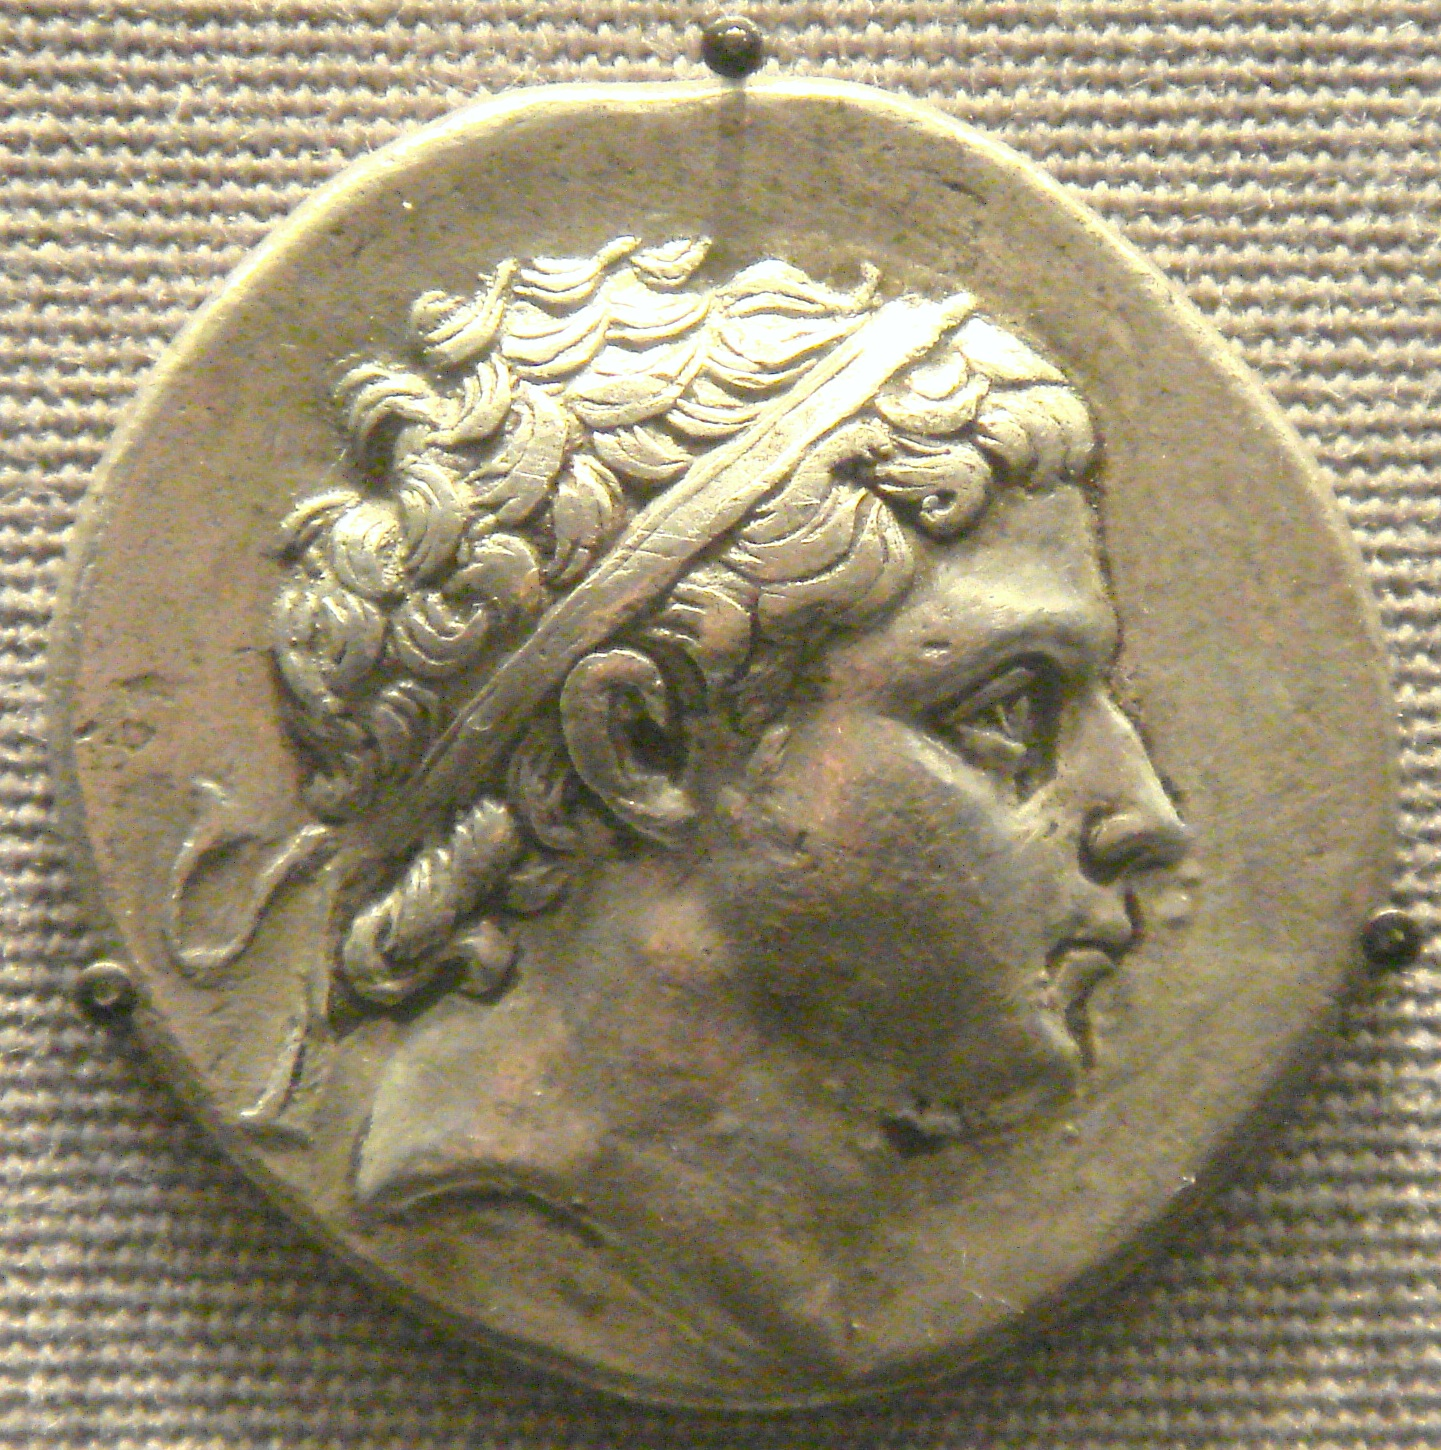
\includegraphics[width=0.40\textwidth]{chast-troya/kiy-prussia/Prusias_I_of_Bithynia.jpg}
\end{center}

\begin{center}
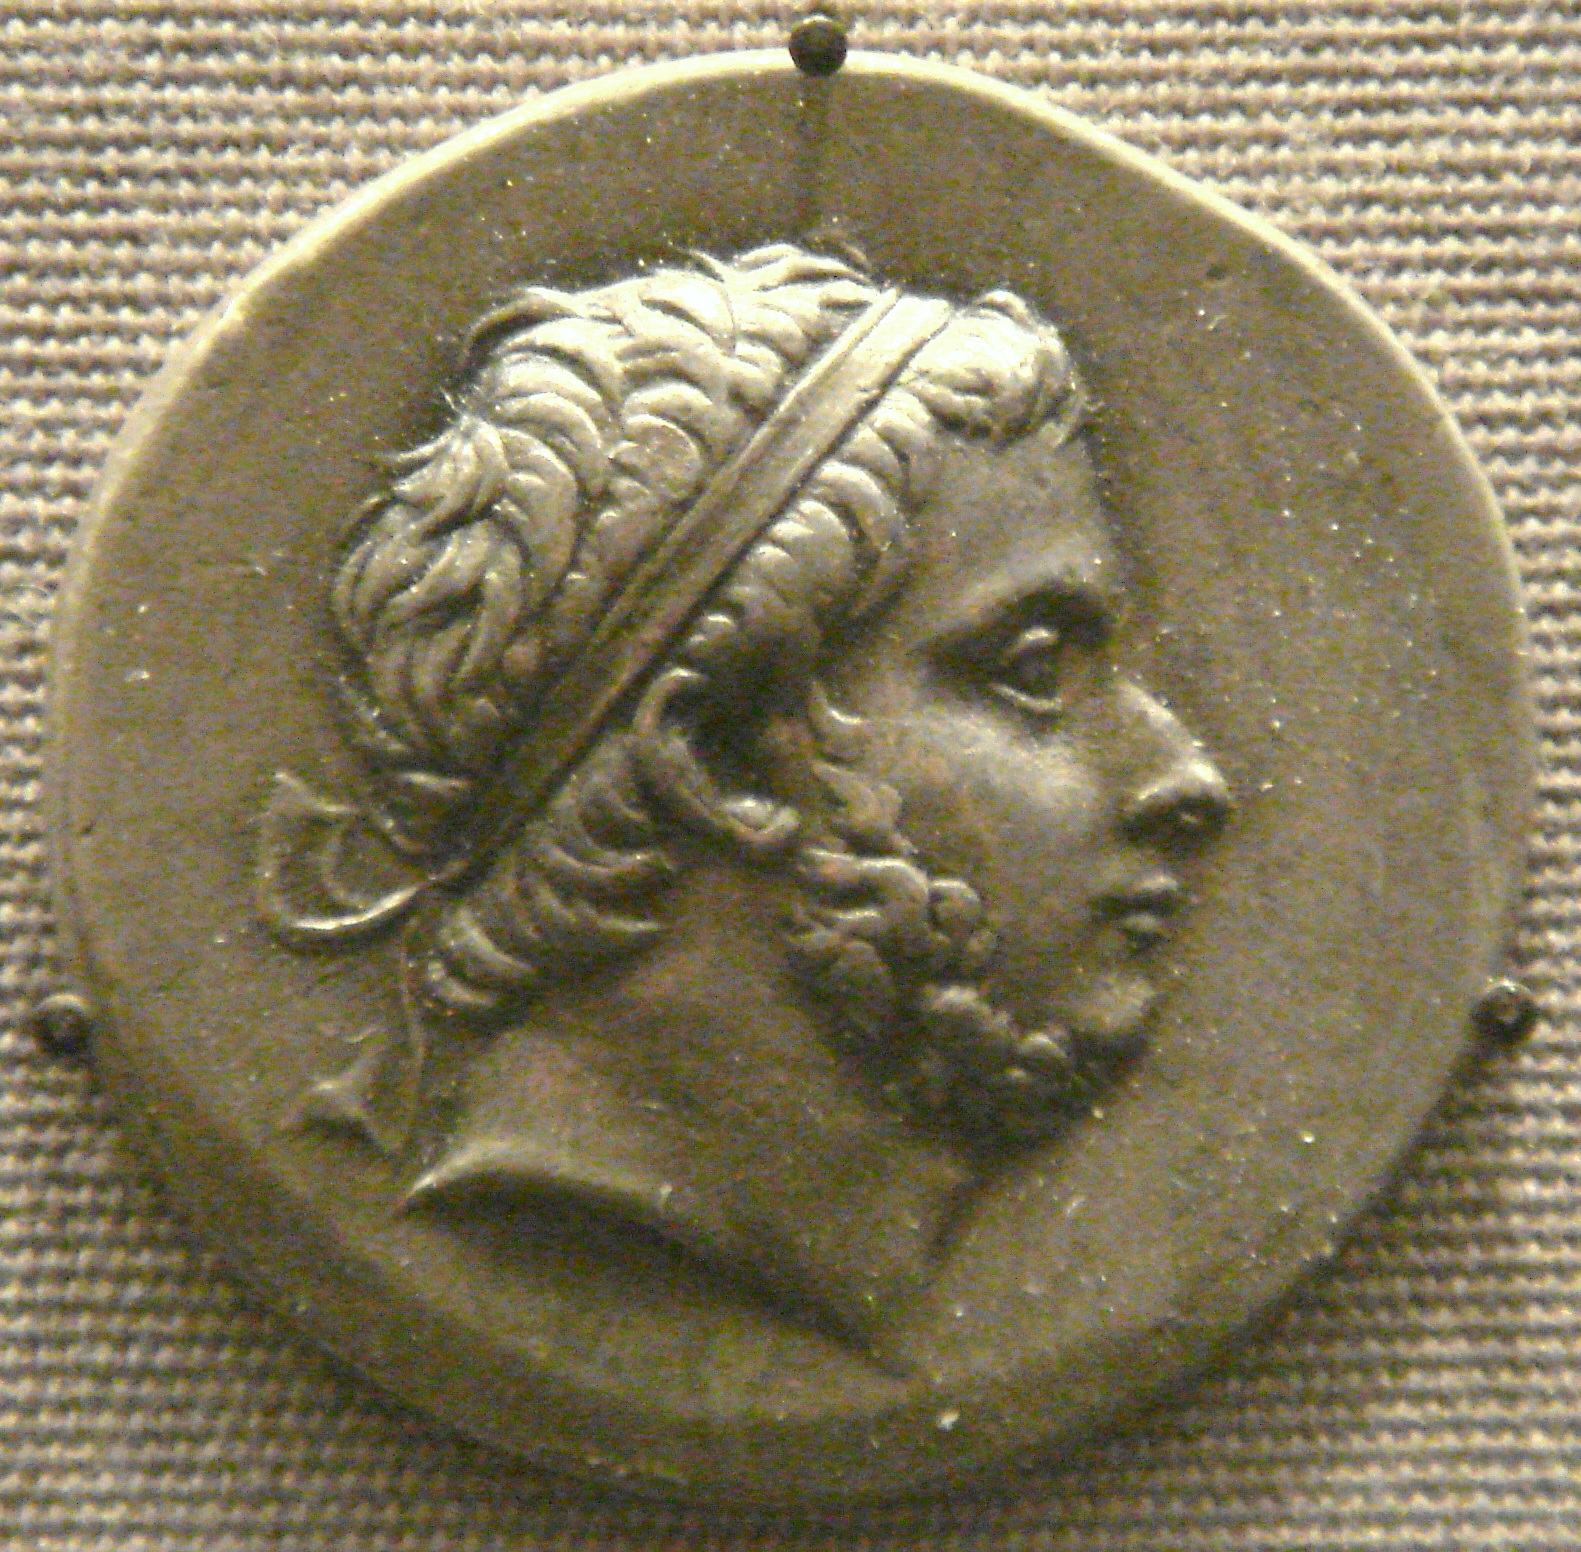
\includegraphics[width=0.40\textwidth]{chast-troya/kiy-prussia/Prusias_I_of_Bithynia_bearded.jpg}
\end{center}

Глядишь и думаешь – тогда все ходили курчавые, в тогах и с лентами на волосах. Но смотришь на монеты Петра I – а он тоже изображен курчавым да в лавровом венке. И на копеечных монетах Петра I выбит конный греческий воин с копьем. Попробуй по такой монете, не зная, когда и в какой стране жил Петр I, датировать ее.

\begin{center}
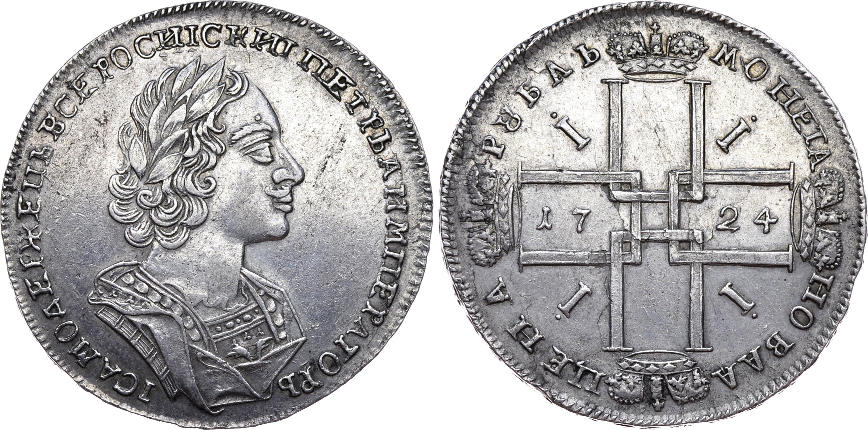
\includegraphics[width=0.60\textwidth]{chast-troya/kiy-prussia/s-04-286_k650.jpg}

\textit{1 рубль 1724 года.}
\end{center}

\begin{center}
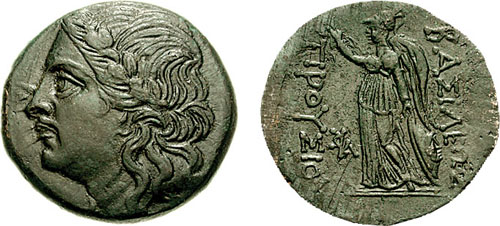
\includegraphics[width=0.60\textwidth]{chast-troya/kiy-prussia/RecGen_16-4.jpg}

\textit{Монета Пруса I.}
\end{center}

Относительно последней монеты некоторые нумизматы полагают, что изображен Аполлон, хотя там явно пожилой Прус I. Несмотря на портретное сходство с ним, Петр I всё же из рода Романовых, а будь он Рюрикович – тогда другое дело, открытие века.

Портреты могут быть разными. Прус II, сын Пруса I, показан на следующей картинке из книги 1413-1415 годов. Прямо Иван Грозный какой-то!

\begin{center}
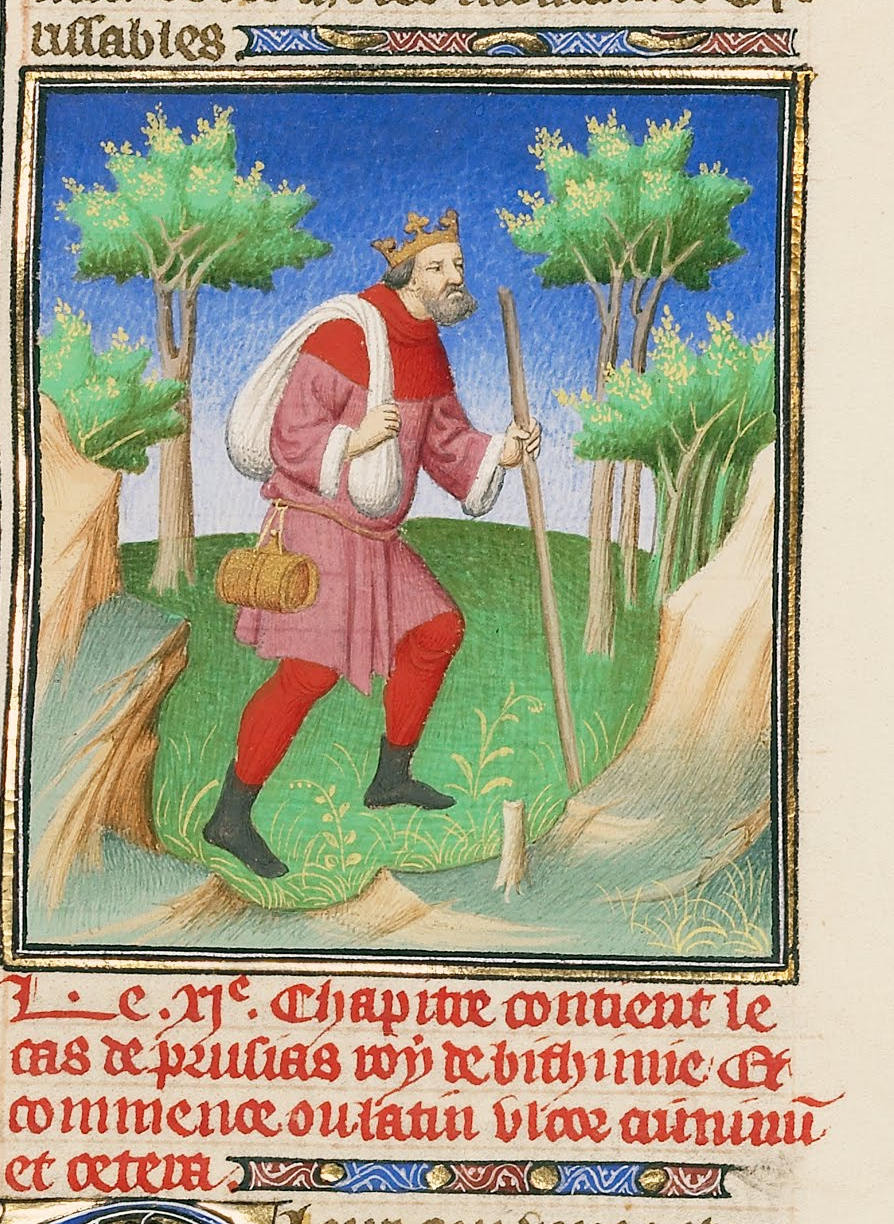
\includegraphics[width=0.92\textwidth]{chast-troya/kiy-prussia/prus2.jpg}
\end{center}

По какой моде одевались, стриглись и брились Прус I и Прус II? Так ли давно они жили относительно 1413 года, как считают ученые?

Вспомним теперь, где по летописям обитали варяги. От моря Варяжского до предела Симова. Напомню и Сказание о Словене и Русе, где приведена грамота Александра Македонского:

\begin{quotation}
Александр, царь царем и над цари бичь божий, презвитяжный рыцарь, всего света обладатель и всех, иж под солнцем, грозный повелитель, к покорным же мне милосердый пощадитель, к непокорным же яростный мечь, страх всего света, честнейший над честнейшими, в далекоразстоятельном и незнаемом крае вашем от нашего величества честь и мир и милость вам и по вас храбросердому народу словенскому, зацнейшему колену русскому великим князем и владцом от моря Варяжского и до моря Хвалимского, велебным и милым мне храбрственному Великосану, мудрому Асану, счастному Авехасану вечне поздравляю, яко самех вас лицем к лицу любезне целую, сердечно приемлю яко други по сердцу моему и нагреднейшии подданицы нашему величеству и сию милость даю вашему владычеству. Аще каковый народ вселится в пределех вашего княжества от моря Варяжскаго и даже до моря Хвалимского, да будут вам и потомку вашему подлежимы вечной работе, во иныя ж пределы отнюдь да не вступит нога ваша. Сие достохвалное дело замкнено сим нашим листом и подписано нашею цысарскою высокодержавною правицею и за природным нашим государьским златокованным гербом привешеным.[...]
\end{quotation}

Границы княжества Великосана, Асана, Авехасана определены между морем Варяжским и морем Хвалимским. Хвалимское – Каспийское. А если предположить, что Варяжским, кроме Балтийского, слыло и Средиземное? 

От Каспия до Средиземного – более правдоподобно, чем от Каспия до Балтийского. Да и Кавказские горы в некоторых летописях связывают с Уграми. А скифские князья Словен и Рос переселились с родами своими откуда? От Евксинпонта, от Черного моря – оно ведь между Каспийским и Средиземным. Оттуда и стали расселяться в другие края.

И если разобрать предложение, что Рюрика призывали из города Прусы, то, принимая за них таковой город в Малой Азии, то в самом деле получится, что «за морем».

Более этого предполагать не стану. Слишком много противоречий.

У меня сложилось впечатление, что в летописной истории произошла путаница с привязкой предметов и событий к пространству и времени. Я бы мог подумать, что на бумаге произошло «раздвоение» городов и местностей, однако оно существует в действительности. 

На юге Черного моря – город Пруса (Бурса), названное от Пруса. На юге Балтийского – жили Прусы, правил ими Прус. Балтийское море слыло Варяжским, но и Черное море по некоторым прикидкам, о которых я уже говорил – тоже Варяжским. И там жили Прусии – жители Прусы и окрестностей. И правил ими Прус.

Мы забрались с такие дебри истории, выйти из которых, кажется, обычный образ мыслей и стройная логика не помогут.

Но странная связь нашего Киева и Трои продолжается.
